\chapter{Real-time komunikace}
Real-time komunikace představuje významný prvek v aplikacích, kde je zapotřebí velmi rychlých reakcí systému. Zpravidla se za real-time aplikaci považuje systém, který řeší časové korekce posílaných signálů a tedy vzájemnou časovou synchronizaci vysílače a přijímače. Obecně lze však za real-time aplikaci uvažovat systém, který reaguje na požadavky bez zbytečného dopravního zpoždění, které je například u webových aplikací naprosto běžné. Předejít však dopravnímu zpoždění u webových aplikací není možné. Důvod je prostý. Webová aplikace musí být dostupná pro všechny uživatele na celém světě a z toho plyne, že každý uživatel je na jiném geografickém místě a čas potřebný k dostání informace ke koncovým uživatelům není stejný. Tento problém lze částečně vyřešit distribuovaným systémem, kdy se servery přibližují uživatelům, což prakticky dělají například streamovací portály jako je YouTube. Toto řešení má svá omezení a proto druhým způsobem, jak ušetřit čas při komunikaci s koncovým prvkem, je zjednodušit komunikační protokol, nebo se omezit na co nejméně zbytečné režie a to i za tu cenu, že nedojde ke stoprocentnímu přenosu informace.

\section{Hardwarové prostředky senzorické sítě}
Hardwarové prostředky této sítě nejsou v současné chvíli nijak přesně definovány. Je tedy možné síť navrhnout libovolným způsobem. Vzhledem ke komplikovanosti celé problematiky bude tato síť striktně metalická paketová. Taková síť se tedy skládá v nejmenší konfiguraci pouze z koncového členu a serveru. S narůstajícím počtem koncových členů je zapotřebí síť patřičně rozšiřovat. Výhodou tohoto systému je fakt, že se daná síť nijak neliší od běžných metalických ethernetových sítí, tzn. že lze využít veškeré dostupné prostředky pro tvorbu této sítě a není zapotřebí vyvíjet zbytečně drahá nová zařízení.

Celá síť se tak skládá z klasického ethernetového vedení a rozbočovačů, přepínačů popř. směrovačů. Zbývá tedy vyřešit server a koncové členy. Zde však záleží na praktické aplikaci. Vezmeme-li však v úvahu nejobyčejnější systém, server pak může být prakticky jakýkoliv počítač, který dokáže zpracovat příchozí požadavky. Tzn. musí být dostatečně výkonný a pro lepší bezpečnost celého systému také redundantní (nebo alespoň některé kritické komponenty v něm). Redundanci komponent však dobře řeší klasické servery, kde jsou redundantní například zdroj, pevné disky, řadiče a dále duální paměti popř. procesory.

Samotné koncové prvky se pak sestávají z nízkoodběrových procesorů, které mají menší, pro danou aplikaci však dostatečný výkon. Zde opět záleží na daném účelu koncového zařízení. Pokud má sloužit jako koncentrátor, tedy zařízení sbírající data ze senzorů, potřebuje větší výkon než například termální čidlo. Výkon koncového prvku je tak dán samotným programem, který na tomto prvku poběží.

Tato síť je tedy v takovém stavu, kdy je zapojen server (nejlépe na nezávislém napájení) a senzory jsou zapojeny v ethernetové síti pomocí běžných síťových prvků. Důležité je však vyřešit co se stane, když vypadne napájení? V tomto okamžiku síť prakticky přestane fungovat. Toto se nijak neliší od např. běžné zapojení elektroinstalace. Sice by šlo zajistit napájení koncových prvků, protože server může být zapojen na více nezávislých zdrojích elektrické energie, to však nebude např. v rodinném domě běžné. Horší případ nastane, když vypadne připojení k internetu. Zde by se nejednalo o problém, pokud by se server nacházel v řízeném objektu. Jediný efekt by byl ten, že by nebylo možné server ovládat vzdáleně. Horší situace ovšem nastane v okamžiku, kdy je server umístěn ve vzdálené serverovně. V takovém případě je pro tuto senzorickou síť potřeba vyřešit tzv. disaster solution, tedy nějaký fallback zařízení při selhání. Samotné koncové členy musí vědět jak se chovat bez příchozího signálu. To většinou není problém, protože paradoxně není většinou potřeba řešit jejich chování. To je nutné pouze v případě zabezpečení objektů. Starostí koncových členů totiž není např. vypnout světlo, pokud není přítomen signál. V takovém objektu je však zapotřebí zařadit do sítě zařízení, které bude přijímat od serveru povely a obsluhovat síť. V případě přerušení spojení se serverem převezme toto zařízení kontrolu nad sítí a uvede objekt do dočasného módu, než se problém vyřeší, nebo než přijede servis. Bude tak možné i nadále ovládat alespoň na základní úrovni většinu zařízení.

\section{Real-time ve webových aplikacích}
Ve webových aplikacích žádný real-time jako takový v podstatě neexistuje. 
%TODO AJAX, websocket

\section{TCP}
Protokol TCP je jedním ze dvou transportních protokolů, které tento systém využívá.
%TODO Co to je, jak to funguje a k čemu je to dobré.
\begin{figure}[h]
    \centering
	\makebox[\textwidth]{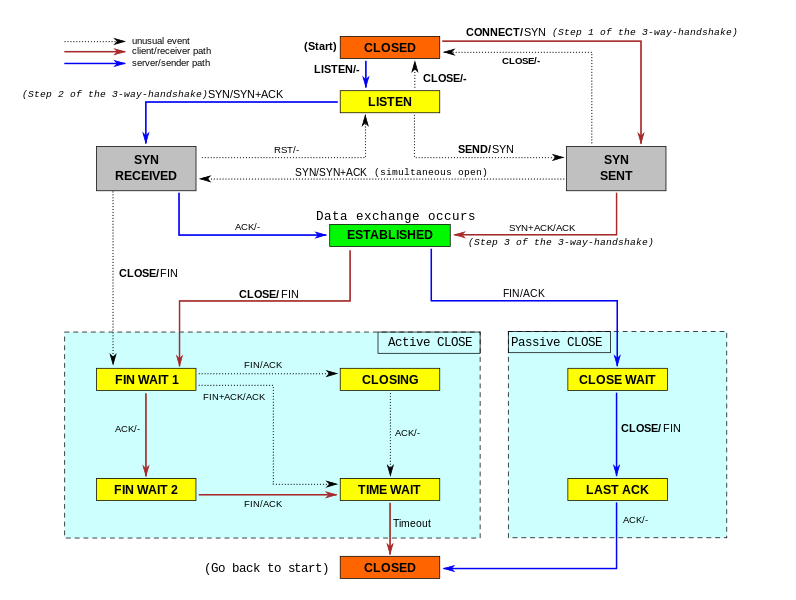
\includegraphics[width=\textwidth]{img/tcp.png}}
	\caption{TCP stavový diagram} %TODO zdroj http://commons.wikimedia.org/wiki/File:Tcp_state_diagram_fixed_new.svg
    %\label{fig:awesome_image}
\end{figure}

\section{UDP}